%%%%%%%%%%%%%%%%%%%%%%%%%%%%%%%%%%%%%%%%%
% Beamer Presentation
% LaTeX Template
% Version 1.0 (10/11/12)
%
% This template has been downloaded from:
% http://www.LaTeXTemplates.com
%
% License:
% CC BY-NC-SA 3.0 (http://creativecommons.org/licenses/by-nc-sa/3.0/)
%
%%%%%%%%%%%%%%%%%%%%%%%%%%%%%%%%%%%%%%%%%

%----------------------------------------------------------------------------------------
%	PACKAGES AND THEMES
%----------------------------------------------------------------------------------------

\documentclass{beamer}

\mode<presentation> {
\usetheme{Copenhagen}
%\usecolortheme{whale}
}
\setbeamertemplate{headline}{}
\setbeamertemplate{navigation symbols}{}
\setbeamertemplate{footline}{}

\usepackage{graphicx} % Allows including images
\usepackage{booktabs} % Allows the use of \toprule, \midrule and \bottomrule in tables

\usepackage{xcolor}

\usepackage{listings} % Source code listingse

\usepackage[utf8]{inputenc}
\usepackage[ngerman]{babel}
\usepackage{hyperref}

\definecolor{darkgreen}{rgb}{0,0.5,0}



 
\lstset{language=C++,
                basicstyle=\small,
                keywordstyle=\color{blue}\ttfamily,
                stringstyle=\color{red}\ttfamily,
                commentstyle=\color{darkgreen}\ttfamily,
                morecomment=[l][\color{magenta}]{\#},
                breaklines=true
                breakwhitespaces=true
}

\AtBeginSection[]{
  \begin{frame}
  \vfill
  \centering
  \begin{beamercolorbox}[sep=8pt,center,shadow=true,rounded=true]{title}
    \usebeamerfont{title}\insertsectionhead\par%
  \end{beamercolorbox}
  \vfill
  \end{frame}
}


\title[Graphen II]{ICPC Teilnehmervortrag: Graphenalgorithmen II} % The short title appears at the bottom of every slide, the full title is only on the title page

\author{Markus Schneckenburger, Moritz Uehling, Florian Weber, Cora Weidner } % Your name
\institute[UCLA] % Your institution as it will appear on the bottom of every slide, may be shorthand to save space
{
	KIT\\ICPC-Teilnehmervortrag
}
\date{28.05.15} % Date, can be changed to a custom date

\begin{document}

\begin{frame}
\titlepage % Print the title page as the first slide
\end{frame}

\begin{frame}
\frametitle{Übersicht} 
\tableofcontents
\end{frame}

\begin{frame}
\frametitle{Code und mehr} 
Den kompletten Code (inklusive dem der Folien) findet ihr unter: 

\url{https://github.com/Florianjw/ICPC-Graphen}

\end{frame}


%\include{examples}

%-----------------------------
\section{MST und Kruskal}
\subsection{MST}

\begin{frame}
\frametitle{Minimum Spanning Tree (MST)}
\begin{itemize}
\item "finde das billigste Netzwerk"
\item genau: \\
Gegeben sei ein zusammenhängender ungerichteter gewichteter Graph, gesucht ist ein zusammenhgängender Teilgraph mit geringstem Gesamtgewicht.
\end{itemize}
\end{frame}

\begin{frame}
\frametitle{Lösung}
\begin{itemize}
\item Ansatz: baue einen Baum mit greedy Algorithmus:
\begin{enumerate}
\item betrachte Kante mit niedrigstem Gewicht
\item untersuche: führt hinzufügen der Kante zu einem Zyklus?
\begin{itemize}
\item Ja: verwerfe Kante
\item Nein: füge Kante zum Baum hinzu
\end{itemize}
\item starte bei 1. mit restlichen Kanten bis alle abgearbeitet sind
\item $ \implies $ Baum ist ein MST
\end{enumerate}
\end{itemize}
\end{frame}

\begin{frame}
\frametitle{Lösung}
\begin{figure}
\includegraphics[width=0.75\linewidth]{kruskal_graphs/graph1.pdf}
\end{figure}
\end{frame}

\section{SSSP (Single Source Shortest Path)}
\subsection{Dijkstra}
\begin{frame}
\frametitle{Das Problem}
\begin{block}{Das Problem}
Breitensuche schlägt bei gewichteten Graphen fehl.
\end{block}
\end{frame}

\begin{frame}
\frametitle{Das Problem}
\begin{figure}
\includegraphics[scale=.8]{dijkstra_graphs/bfs_fail_0.pdf}
\end{figure}
\end{frame}

\begin{frame}
\frametitle{Das Problem}
\begin{figure}
\includegraphics[scale=.8]{dijkstra_graphs/bfs_fail_1.pdf}
\end{figure}
\end{frame}

\begin{frame}
\frametitle{Das Problem}
\begin{figure}
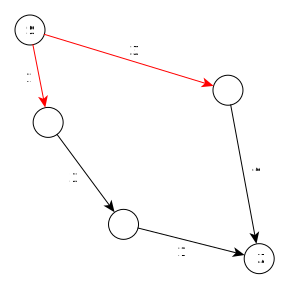
\includegraphics[scale=.8]{dijkstra_graphs/bfs_fail_2.pdf}
\end{figure}
\end{frame}

\begin{frame}
\frametitle{Das Problem}
\begin{figure}
\includegraphics[scale=.8]{dijkstra_graphs/bfs_fail_3.pdf}
\end{figure}
\end{frame}

\begin{frame}
\frametitle{Das Problem}
\begin{figure}
\includegraphics[scale=.8]{dijkstra_graphs/bfs_fail_4.pdf}
\end{figure}
\end{frame}

\begin{frame}
\frametitle{Das Problem}
\begin{figure}
\includegraphics[scale=.8]{dijkstra_graphs/bfs_fail_4.pdf}
\end{figure}

$\implies$ Es wird ein Weg der Länge $7$ gefunden, obwohl $5$ das Optimum ist

\end{frame}


\begin{frame}
\frametitle{Djikstras Algorithmus}
\begin{itemize}
\item Grundsätzliche Idee: Breitensuche mit Priortiy-Queue (so dass "nähere" Knoten zuerst behandelt werden)
\item \lstinline|std::priority_queue| verwendet binären Heap
\item $\implies$ Laufzeit von Dijkstra ist $\Theta((n + m) \log n)$
\item Nachteil: Funktioniert nicht bei negativen Kantengewichten
\end{itemize}
\end{frame}

\begin{frame}[fragile]
\frametitle{Code}
Header: 
\begin{lstlisting}[basicstyle=\tiny]
#include<vector>
#include<algorithm>
#include<queue> // not priority_queue!
#include<iostream>

using namespace std;

struct arrival_event {
  int to;
  int weight;
};


bool operator < (const arrival_event& e1, const arrival_event& e2) {
	   // inversed
    return e1.weight > e2.weight;
}
\end{lstlisting}

\end{frame}

\begin{frame}[fragile]
\frametitle{Code}
\begin{lstlisting}[basicstyle=\tiny]
vector<int> dijkstra(vector<vector<arrival_event>>& nodes, int startnode) {
  vector<int> distances (nodes.size(), 2000000000);

  priority_queue<arrival_event> todo;

  todo.push({startnode, 0});

  while(!todo.empty()) {
    auto current = todo.top();
    todo.pop();

    if(current.weight < distances[current.to]) {
      distances[current.to] = current.weight;

      for(int i = 0; i < nodes[current.to].size(); i++) {
        arrival_event next = nodes[current.to][i];
        next.weight += current.weight;

        todo.push(next);
      }
    }
  }

  return distances;
}
\end{lstlisting}

\end{frame}


\begin{frame}
\frametitle{Beispiel}
\begin{figure}
\includegraphics[scale=.8]{dijkstra_graphs/dijkstra_0.pdf}
\end{figure}
\end{frame}

\begin{frame}
\frametitle{Beispiel}
\begin{figure}
\includegraphics[scale=.8]{dijkstra_graphs/dijkstra_1.pdf}
\end{figure}
\end{frame}

\begin{frame}
\frametitle{Beispiel}
\begin{figure}
\includegraphics[scale=.8]{dijkstra_graphs/dijkstra_2.pdf}
\end{figure}
\end{frame}

\begin{frame}
\frametitle{Beispiel}
\begin{figure}
\includegraphics[scale=.8]{dijkstra_graphs/dijkstra_3.pdf}
\end{figure}
\end{frame}

\begin{frame}
\frametitle{Beispiel}
\begin{figure}
\includegraphics[scale=.8]{dijkstra_graphs/dijkstra_4.pdf}
\end{figure}
\end{frame}

\begin{frame}
\frametitle{Beispiel}
\begin{figure}
\includegraphics[scale=.8]{dijkstra_graphs/dijkstra_5.pdf}
\end{figure}
\end{frame}

\begin{frame}
\frametitle{Beispiel}
\begin{figure}
\includegraphics[scale=.8]{dijkstra_graphs/dijkstra_6.pdf}
\end{figure}
\end{frame}

\begin{frame}
\frametitle{Beispiel}
\begin{figure}
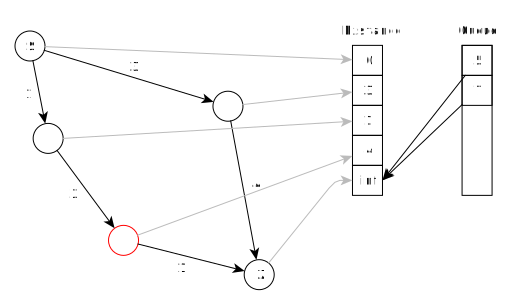
\includegraphics[scale=.8]{dijkstra_graphs/dijkstra_7.pdf}
\end{figure}
\end{frame}

\begin{frame}
\frametitle{Beispiel}
\begin{figure}
\includegraphics[scale=.8]{dijkstra_graphs/dijkstra_8.pdf}
\end{figure}
\end{frame}

\begin{frame}
\frametitle{Beispiel}
\begin{figure}
\includegraphics[scale=.8]{dijkstra_graphs/dijkstra_9.pdf}
\end{figure}
\end{frame}

\begin{frame}
\frametitle{Beispiel}
\begin{figure}
\includegraphics[scale=.8]{dijkstra_graphs/dijkstra_A.pdf}
\end{figure}
\end{frame}

\begin{frame}
\frametitle{Beispiel}
\begin{figure}
\includegraphics[scale=.8]{dijkstra_graphs/dijkstra_B.pdf}
\end{figure}
\end{frame}
\begin{frame}{Übersicht}

\begin{itemize}
\itemsep1pt\parskip0pt\parsep0pt
\item
  Problem: Dijkstra kommt nicht mit negativen Kanten zurecht
\end{itemize}

\begin{figure}[htbp]
\centering
\includegraphics[width=\linewidth]{dijkstra_gegenbeispiel.pdf}
\end{figure}

\end{frame}

\begin{frame}{Ansätze}
\begin{itemize}
\item
  Lösung: rohe %\sout{Gewalt}
  Rechenleistung
\item
  Wichtige Einschränkung: negative Kreise auf irgendeinem Pfad von
  \texttt{Q} zu \texttt{S} bedeuten Nichtexistenz eines kürzesten Pfades
\item
  Idee 1: vollständige Tiefensuche.

  \begin{itemize}
  \item
    selbst für Brute-Force-Verhältnisse zu langsam (exponentielle
    Laufzeit)
  \end{itemize}
\end{itemize}
\end{frame}
\begin{frame}{Ansätze}
\begin{itemize}
\item
  Idee 2:
  \begin{itemize}
  \item
    kürzester Pfad enthält maximal $|V| - 1$ Kanten
  \item
    Enthalte der kürzeste Pfad $i$ Kanten. Falls wir alle kürzesten
    Pfade mit bis zu $i - 1$ Knoten kennen:

    \begin{itemize}
    \item
      Zu den kürzesten Pfaden mit bis zu $i$ Kanten fehlt höchstens eine
      Kante.
    \item
      Probiere für alle Kanten, ob sie irgendwo einen kürzeren Pfad
      erzeugen
    \end{itemize}
  \item
    Für $i = 0$ ist die Distanz der Quelle zu sich selbst 0, und die zu
    allen anderen Knoten $\inf$
  \end{itemize}
\item
  Idee 2 ist offensichtlich vielversprechender, sie führt zum
  Algorithmus von Belllman und Ford.
\end{itemize}
\end{frame}

\begin{frame}{Initialisierung}
\begin{figure}[htbp]
\centering
\includegraphics[width=\linewidth]{bellman_ford_graphs/graph_00.pdf}
\end{figure}
\end{frame}

\begin{frame}{Runde 1}
\begin{figure}[htbp]
\centering
\includegraphics[width=\linewidth]{bellman_ford_graphs/graph_01.pdf}
\end{figure}
\end{frame}


\begin{frame}{Runde 1}
\begin{figure}[htbp]
\centering
\includegraphics[width=\linewidth]{bellman_ford_graphs/graph_02.pdf}
\end{figure}
\end{frame}

\begin{frame}{Runde 1}
\begin{figure}[htbp]
\centering
\includegraphics[width=\linewidth]{bellman_ford_graphs/graph_03.pdf}
\end{figure}
\end{frame}

\begin{frame}{Runde 1}
\begin{figure}[htbp]
\centering
\includegraphics[width=\linewidth]{bellman_ford_graphs/graph_04.pdf}
\end{figure}
\end{frame}

\begin{frame}{Runde 1}
\begin{figure}[htbp]
\centering
\includegraphics[width=\linewidth]{bellman_ford_graphs/graph_05.pdf}
\end{figure}
\end{frame}

\begin{frame}{Runde 1}
\begin{figure}[htbp]
\centering
\includegraphics[width=\linewidth]{bellman_ford_graphs/graph_06.pdf}
\end{figure}
\end{frame}

\begin{frame}{Runde 2}
\begin{figure}[htbp]
\centering
\includegraphics[width=\linewidth]{bellman_ford_graphs/graph_07.pdf}
\end{figure}
\end{frame}

\begin{frame}{Runde 2}
\begin{figure}[htbp]
\centering
\includegraphics[width=\linewidth]{bellman_ford_graphs/graph_08.pdf}
\end{figure}
\end{frame}

\begin{frame}{Runde 2}
\begin{figure}[htbp]
\centering
\includegraphics[width=\linewidth]{bellman_ford_graphs/graph_09.pdf}
\end{figure}
\end{frame}

\begin{frame}{Runde 2}
\begin{figure}[htbp]
\centering
\includegraphics[width=\linewidth]{bellman_ford_graphs/graph_10.pdf}
\end{figure}
\end{frame}

\begin{frame}{Runde 2}
\begin{figure}[htbp]
\centering
\includegraphics[width=\linewidth]{bellman_ford_graphs/graph_11.pdf}
\end{figure}
\end{frame}

\begin{frame}{Runde 2}
\begin{figure}[htbp]
\centering
\includegraphics[width=\linewidth]{bellman_ford_graphs/graph_12.pdf}
\end{figure}
\end{frame}

\begin{frame}{Runde 2}
\begin{figure}[htbp]
\centering
\includegraphics[width=\linewidth]{bellman_ford_graphs/graph_13.pdf}
\end{figure}
\end{frame}
\begin{frame}{Runde 3 (keine Änderungen $\rightarrow$ fertig)}

\begin{figure}[htbp]
\centering
\includegraphics[width=\linewidth]{bellman_ford_graphs/graph_14.pdf}
\end{figure}

\end{frame}

\begin{frame}[fragile]{Code}
\begin{lstlisting}[basicstyle=\footnotesize]
using node = std::size_t;
using dist = double;

struct edge {
    node from;
    node to;
    dist weight;
};

const auto inf_dist = std::numeric_limits<dist>::infinity();
\end{lstlisting}
\end{frame}

\begin{frame}[fragile]{Code}

\begin{lstlisting}[basicstyle=\footnotesize]
std::vector<dist> bellman_ford(
        std::size_t node_count,
        const std::vector<edge>& edges,
        node source
) {
    std::vector<dist> min_dists(node_count, inf_dist);
    min_dists[source] = 0;
    for (std::size_t i = 0; i < node_count + 1; ++i) {
        auto changes = false;
        for(const auto& e: edges) {
            const auto old_dist = min_dists[e.to];
            const auto new_dist = min_dists[e.from]
                                  + e.weight;
            if (new_dist < old_dist) {
                min_dists[e.to] = new_dist;
                changes = true;
            }
        }
        // ...
\end{lstlisting}


\end{frame}

\begin{frame}[fragile]{Code}

\begin{lstlisting}[basicstyle=\footnotesize]
        // ...
        if (!changes) { break; }
        if (i == node_count) {
            throw std::runtime_error{
                "negative cycle"};
        }
    }
    return min_dists;
}
\end{lstlisting}

\end{frame}

\begin{frame}[fragile]{Code}

\begin{lstlisting}[basicstyle=\footnotesize]
int main() try {
    const auto edges = std::vector<edge>{
        {0, 1,  7}, {0, 4,  -1},
        {1, 0, 10}, {1, 3,  -4},
        {2, 4,  1},
        {3, 0,  0}, {3, 2, 2.5},
        {4, 1, 23}
    };
    const auto min_dists = bellman_ford(5, edges, 0);
    std::copy(min_dists.begin(), min_dists.end(),
        std::ostream_iterator<dist>{std::cout, "\n"});
} catch (std::runtime_error& e) {
    std::cerr << "Error: " << e.what() << '\n';
}
\end{lstlisting}

\end{frame}

\begin{frame}{Weitere Eigenschaften}

\begin{itemize}
\itemsep1pt\parskip0pt\parsep0pt
\item
  Negative Kreise lassen sich durch eine weitere Anwendung detektieren
\item
  Negative Kreise die nicht auf dem Weg zum Ziel liegen, verfälschen das
  Ergebnis nicht

  \begin{itemize}
  \itemsep1pt\parskip0pt\parsep0pt
  \item
    Die Detektion aller problemlosen Knoten ist mit $V - 1$ weiteren
    Anwendungen möglich
  \end{itemize}
\end{itemize}

\end{frame}

\begin{frame}{Beurteilung}

\begin{itemize}
\itemsep1pt\parskip0pt\parsep0pt
\item
  Assymptotische Komplexität $\in O(|V| \cdot |E|)$
\item
  Profitiert nicht von kurzen Distanzen zwischen Quelle und Senke
\item
  Relativ leicht zu implementieren
\end{itemize}

\end{frame}

\begin{frame}{Fazit}

\begin{quote}
Kann man schon so machen, meistens will man das aber nicht
\end{quote}

\end{frame}

%------------------------------------------------
\section{All Pairs Shortest Paths (APSP)} 

\subsection{Idee} 

\begin{frame}
\frametitle{APSP - All Pairs Shortest Paths}
\begin{block}{Problemstellung}
Man hat einen Graphen gegeben, der gewichtet ist. Nun möchte man den kürzesten Pfad zwischen allen Knoten i zu allen Knoten j herausfinden.
\end{block}
\end{frame}

%------------------------------------------------

\begin{frame}
\frametitle{APSP - Erster Ansatz}
\begin{block}{Lösungsansatz}
Man verwendet den bereits bekannten SSSP-Algorithmus, und führe diesen nach bedarf aus, d.h. in diesem Fall n-mal.
\end{block}

\begin{block}{Laufzeit}
$n \cdot O (m + n \cdot log(n))$\\$
= n \cdot O (n^2 + n \cdot log(n))$\\$ 
= n \cdot O (n^2 + n^2) $\\$ 
= O (n^3) $\\
$\implies$ geht es einfacher in etwa der selben Zeit?
\end{block}
\end{frame}

%------------------------------------------------

\begin{frame}
\frametitle{APSP - Zweiter Ansatz}
\begin{block}{Lösungsansatz}
Wir wissen: jeder Pfad zwischen zwei Knoten ist entweder bereits der kürzeste, oder es gibt einen Kürzeren Pfad als zwei Verknüpfung anderer Pfade über mindestens einen dritten Knoten.
\end{block}

\begin{block}{Genauer}
Systematisch in einer Adjazenzmatrix A:
Nehme für jeden Pfad $A[i][j] = \min\left(A[i][j], A[i][k] + A[i][k]\right)$, d.h. entweder der Pfad ist bereits minimal, oder ein Pfad über Knoten k ist kürzer und wird als neues Minimum übernommen.
Wenn man nun richtig iteriert, erhält man alle minimalen Pfade.
\end{block}
\end{frame}

%------------------------------------------------

\subsection{Code}

\begin{frame}[fragile] % Need to use the fragile option when verbatim is used in the slide
\frametitle{Code}

\begin{lstlisting}
for (int k = 0; k < V; k++)
    for (int i = 0; i < V; i++)
        for (int j = 0; j < V; j++)
            A[i][j] = min(
              A[i][j],
              A[i][k] + A[k][j]
            );
\end{lstlisting}

~\\$\implies$ der Aufwand liegt in $O(n^3)$

\end{frame}

%------------------------------------------------

\begin{frame}
\frametitle{Beispiel - Urzustand}

\includegraphics[width=\linewidth]{floyd_warshall_graphs/graph1.JPG}

\end{frame}

%------------------------------------------------

\begin{frame}
\frametitle{Beispiel - Über Knoten A}

\includegraphics[width=\linewidth]{floyd_warshall_graphs/graph2.JPG}

\end{frame}

%------------------------------------------------

\begin{frame}
\frametitle{Beispiel - Über Knoten B}

\includegraphics[width=\linewidth]{floyd_warshall_graphs/graph3.JPG}

\end{frame}

%------------------------------------------------

\begin{frame}
\frametitle{Beispiel - Über Knoten C}

\includegraphics[width=\linewidth]{floyd_warshall_graphs/graph4.JPG}

\end{frame}

%------------------------------------------------

\begin{frame}
\frametitle{Beispiel - Über Knoten D (1)}

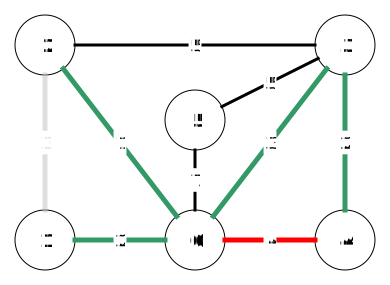
\includegraphics[width=\linewidth]{floyd_warshall_graphs/graph5.JPG}

\end{frame}

%------------------------------------------------

\begin{frame}
\frametitle{Beispiel - Über Knoten D (2)}

\includegraphics[width=\linewidth]{floyd_warshall_graphs/graph6.JPG}

\end{frame}

%------------------------------------------------

\begin{frame}
\frametitle{Beispiel - Über Knoten D (3)}

\includegraphics[width=\linewidth]{floyd_warshall_graphs/graph7.JPG}

\end{frame}

%------------------------------------------------

\begin{frame}
\frametitle{Beispiel - Über Knoten D (4)}

\includegraphics[width=\linewidth]{floyd_warshall_graphs/graph8.JPG}

\end{frame}

%------------------------------------------------

\begin{frame}
\frametitle{Beispiel - Über Knoten D (5)}

\includegraphics[width=\linewidth]{floyd_warshall_graphs/graph9.JPG}

\end{frame}

%------------------------------------------------

\begin{frame}
\frametitle{Beispiel - Über Knoten D (6)}

\includegraphics[width=\linewidth]{floyd_warshall_graphs/graph10.JPG}

\end{frame}

%------------------------------------------------

\begin{frame}
\frametitle{Weitere Anwendungen}
\begin{itemize}

\item Auch für SSSP - Probleme anwendbar (wenn $\vert V \vert < 400$)
\item Detektion von negativen oder günstigsten Zyklen möglich $\implies$ ein negativer Zyklus existiert genau dann, wenn ein Diagonaleintrag negativ ist
\item Finden des Durchmessers eines Graphen (der längste der kürzesten Pfade)
\item Minimax, die kleinsten Maximalkosten von allen Wegen
\item Maximin, die größten Minimalkosten von allen Wegen
\end{itemize}
\end{frame}

%------------------------------------------------

\subsection{Beurteilung} 

\begin{frame}
\frametitle{Beurteilung}
\begin{itemize}

\item[+] Asymptotische Komplexität $\in O(n^3)$  und mit Speicher $\in O(n^2)$
\item[+] Sehr leicht zu implementieren (Vierzeiler)
\item[+] Für andere Probleme günstig anzuwenden, wenn $|V|< 400$
\item[-- --] Für andere Probleme \textbf{nur} günstig anzuwenden, wenn $|V|< 400$
\end{itemize}

$\implies$ Gut für das ursprüngliche Problem\\
$\implies$ Auch nützlich für andere Probleme, solange $|V| < 400$
\end{frame}

%------------------------------------------------

\section{Zusammenfassung}

\begin{frame}
\frametitle{Zusammenfassung}
\footnotesize{\begin{table}
\begin{tabular}{l l l l}
\toprule
\textbf{Kriterium} & \textbf{Dijkstra} & \textbf{Bellman Ford} &\textbf{Floyd Warshall}\\
\midrule
Laufzeit & $O((n+m)\log(n))$ & $O(n \cdot m)$ & $O(n^3)$ \\
Max. Größe  & $n,m \leq 300K$ & $n \cdot m \leq 10M$ & $n \leq 400$ \\
Ungewichtet & Ja & Ja (schlecht) & Ja (kleine Graphen) \\
Gewichtet & Ja & Ok & Ja (kleine Graphen) \\
Neg. Kanten & Nein & Ja & Ja \\
Neg. Zyklen & Nein & Ja & Ja \\
Kleine Graphen & Overkill & Overkill & Bestes \\
Kann SSSP? & Ja & Ja & Eingeschränkt \\
\bottomrule
\end{tabular}
\caption{Übersicht}
\end{table}}
Erinnerung: $n:= |V|$ und $m:= |E|$
\end{frame}

%------------------------------------------------


\end{document}
